\chapter{Asking a Private Equity Millionaire How He Got Rich}

This School of Hard Knocks interview, curated by LazyingArt LLC for Video2Book, is not a blackboard lecture in the usual sense. Still, it has a definite analytic spine. We are led from a viral claim about private equity into a sequence of increasingly precise questions about career formation, capital allocation, analytics, sales structure, family life, daily habits, solitude, recovery after loss, and finally legacy. Because the speaker gives us almost no literal formalism, we will write down a cautious companion mathematics whose purpose is not to replace the interview, but to make explicit the commercial logic that the interview keeps uncovering.

\begin{remark}
There are no validated lecture-board equations or diagrams for this chapter. Every formula below is therefore a companion reconstruction from the spoken argument. We use notation only where it sharpens the mechanism and we avoid pretending that a blackboard derivation took place when it did not.
\end{remark}

\section{Viral Re-entry and the Long Game}

The hosts do not begin by introducing Mike Kessner from nothing. They reopen a previous case. The earlier clip that went viral was a simple question --- what industry is best for becoming wealthy? --- and Mike's answer was private equity. The interview now re-enters through that old doorway, and Mike immediately offers a curious update: his own son later moved from consulting into a large private-equity firm, and his son-in-law left investment banking to start one. The point is not that the clip caused those moves. The point is that a commercial judgment, once spoken, begins to echo through a larger network of lives.

From there the interview does the necessary thing: it asks how Mike himself got where he is. The answer is not a clean heroic arc. We get LSU, an abandoned baseball ambition, a transfer to Denver, a first recruiting job that lasted only a month, a move through a large company into St.~Louis, then eventually a long career in insurance. There is a wife met in St.~Louis, a move motivated partly by family obligation, and then more than thirty years in the insurance business. The early part of the story is almost deliberately uneven. That is important. The lecture wants to dislodge the fantasy that success begins with a perfect start.

\begin{definition}
We will call \(C_t\) \emph{career capital} at time \(t\). It is not just skill. It is the accumulated stock of competence, relationships, credibility, position, and repeated execution that makes later opportunities easier to seize.
\end{definition}

A cautious companion update rule is
\begin{equation}
C_{t+1}=C_t+\alpha S_t+\beta N_t+\gamma R_t+\delta E_t,
\end{equation}
where \(S_t\) denotes skill, \(N_t\) network quality, \(R_t\) reputation, and \(E_t\) sustained execution. The interview does not give us these symbols, but it does give us the mechanism. Mike says that for his first several years in insurance he did not really know what he was doing. What he did know was that authentic, high-energy people were likely to become successful over time, and that if he stayed near them and played the long game, some of that motion would compound.

We can compress that verbal rule into a more pointed implication:
\begin{equation}
N_t \uparrow \text{ through authentic, high-energy people}
\Longrightarrow
\Pr(\text{future success}\mid t)\uparrow.
\end{equation}
This is the first real law of motion in the interview. It is not a theorem about finance. It is a theorem about commercial proximity. The person who begins with perfect polish may still fail; the person who learns to place himself inside the right stream of people and keeps working may find that time does the heavy lifting.

The story then advances. Mike spends roughly twenty-five years in the long game, encounters a younger CEO in the insurance world, expects perhaps an acquisition, and instead becomes a friend and then a partner in a new phase. The old firm had become a two-thousand-person private-equity roll-up. The new phase, by his account, has been the most enjoyable part of the career. Why? Because the objective has shifted. The money phase is no longer the only phase; coaching younger people and leaving a legacy have entered the system.

\section{Capital Allocation, Luck, and Industry Choice}

The next move in the interview is beautifully placed. Once career capital is on the table, the hosts ask for the best and worst financial decisions. That forces Mike to reveal not merely what he did for a living, but how he thinks under uncertainty.

A minimal wealth update reads
\begin{equation}
W_{t+1}=W_t+Y_t+\Pi_t-L_t,
\end{equation}
with \(W_t\) the stock of wealth, \(Y_t\) earned income, \(\Pi_t\) investment gains or losses, and \(L_t\) living outflows. The interview immediately decomposes \(\Pi_t\) into separate cases:
\begin{equation}
\Pi_t=\Pi_t^{\text{Nautilus}}+\Pi_t^{\text{Coinbase}}+\Pi_t^{\text{home}}+\cdots.
\end{equation}

Nautilus becomes the good case. Mike happens to read about the company shortly before the pandemic, recognizes its connection to home fitness equipment, adds capital, and then benefits from a global event that traps people at home. He calls this luck, and the chapter should preserve that word. This is not presented as a masterpiece of formal forecasting. It is timing, alertness, and good fortune interacting.

Coinbase becomes the obvious losing trade, though one he still holds. The family home is more interesting. Financially, he says it effectively broke even after roughly twenty years. But he refuses to call it a bad life decision, because the house carried memory, neighborhood, and family life. In other words, the lecture quietly introduces a distinction between financial return and lived return. A house can be disappointing as \(\Pi_t^{\text{home}}\) and still be indispensable as part of a good life.

That distinction matters because the hosts then pivot back to industry choice. They explicitly reopen the old viral question: what industry should a young person be looking at now? Mike updates the answer. He says data science. More broadly, he says analytics. He is careful to say that he is not the expert in that field, but he knows what such people do for a firm like his. They crunch data, identify what is trending, and return signals to the older operators who can act on them.

The companion notation is simple:
\begin{equation}
D \rightarrow A \rightarrow T \rightarrow \text{decision},
\end{equation}
where \(D\) denotes data, \(A\) the analytics layer, and \(T\) the trend signals extracted from the data. Mike explicitly compares the process to ``Moneyball.'' That is exactly right. We are not merely collecting information; we are using pattern recognition to improve where attention is placed. The interview is telling us that a good industry choice is often an information-leverage choice.

\section{Sales Architecture: Team, Specialization, and Edge}

Once analytics has been introduced, the lecture narrows from general industry advice to the inner machinery of an actual insurance firm. This is a crucial transition. The interview no longer asks, ``What field is hot?'' It asks, ``What structure inside a field creates an advantage?''

Mike's first answer is negative. Sales is lonely when it is done on an island. That phrase does a great deal of work. It tells us that even if compensation is high, the organizational form may still be bad. He wants young people entering insurance --- and then expands the point to any sales position --- to be on a real team, ideally one that feels almost like sports. The transcript around this point is somewhat noisy, but the intended claim is clear: isolated selling is fragile; team selling is durable.

A useful companion model is
\begin{equation}
Q_{\text{sales}}=f(T,V,M),
\end{equation}
where \(Q_{\text{sales}}\) is sales effectiveness, \(T\) is team cohesion, \(V\) is vertical specialization, and \(M\) is the morale and shared learning that arise when people work together rather than as scattered individuals.

\subsection{Question \& Answer}

\paragraph{Question.} If sales is often thought of as an individual art, why should a team of specialists beat a strong lone generalist?

\paragraph{Answer.} The interview's answer is twofold. First, a real team changes the emotional and learning environment. When you win, there is something to celebrate; when you lose, the loss can be processed and learned from collectively rather than privately. Second, specialization changes the content of the sales conversation. Mike describes a firm with roughly twenty-five sales people and five or six teams, each tied to particular verticals. There are people who can go to a private-equity conference and speak almost as fluently as private-equity professionals. There are hospitality teams, construction teams, and a restaurant team covering about eight hundred restaurants. What matters is not mere enthusiasm. What matters is the ability to enter the client's world already speaking its language.

This can be written schematically as
\begin{equation}
V \uparrow \Longrightarrow \text{domain fluency} \uparrow \Longrightarrow \text{client trust} \uparrow.
\end{equation}
And once trust rises, the space of solutions grows. The seller is no longer a generic broker. He becomes someone who can recognize recurring pain points, name them before the client does, and attach them to concrete precedents from comparable firms.

\paragraph{Companion diagram.}
\begin{figure}
\centering
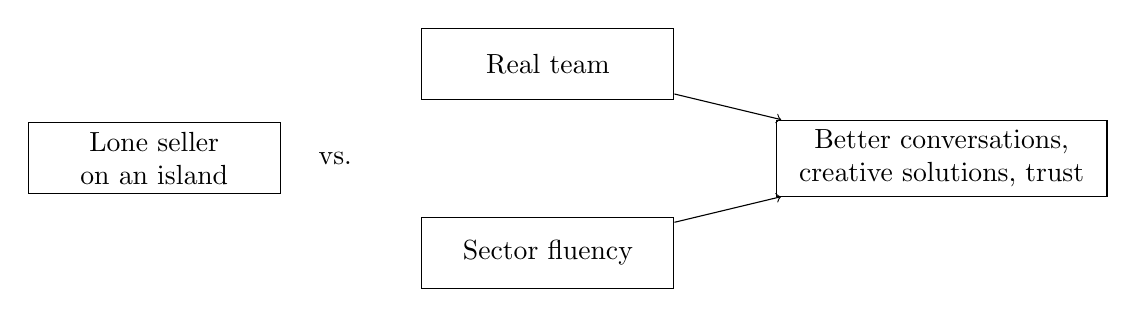
\begin{tikzpicture}[x=1cm,y=1cm]
\node[draw, rectangle, minimum width=3.2cm, minimum height=0.9cm, align=center] (a) at (0,0) {Lone seller\\on an island};
\node[draw, rectangle, minimum width=3.2cm, minimum height=0.9cm, align=center] (b) at (5,1.2) {Real team};
\node[draw, rectangle, minimum width=3.2cm, minimum height=0.9cm, align=center] (c) at (5,-1.2) {Sector fluency};
\node[draw, rectangle, minimum width=4.2cm, minimum height=0.9cm, align=center] (d) at (10,0) {Better conversations,\\creative solutions, trust};
\node at (2.3,0) {vs.};
\draw[->] (b) -- (d);
\draw[->] (c) -- (d);
\end{tikzpicture}
\end{figure}

The diagram is only a reconstruction, but it matches the logic of the interview exactly. The edge is organizational. It is produced by the combination of real team life and real sector knowledge.

\section{Temperament, Family, and the Daily Operating System}

Before the lecture turns inward to habits and mindset, it passes through temperament. Mike says that the most impactful book for him was \textit{Don't Sweat the Small Stuff}. He reads three to five books a month, so the answer matters. He could have reached for a grander title, but he does not. The reason is plain: the book encodes a practical rule about scale. Most perturbations in life are not large enough to justify panic. One must learn to remain calm in chaos.

That is the emotional bridge to the family section. The hosts explicitly say that they have talked about career a lot and now want advice for first-time fathers and husbands. The fatherhood answer is strikingly concrete: quantity of time with children matters. The child should know, when young, that the parent is simply there. In the marriage answer, the advice becomes almost ritualistic. If one comes home from a hard day at work, it may be wise to pull over, take a breath, and remember that the next role begins at the door. Work does not automatically convert into good partnership.

The transcript becomes somewhat corrupted in the next minute, but the underlying claims are still recoverable. He emphasizes affection for spouse and children, even though he does not consider himself naturally affectionate with most people. He recommends humor when humor is natural, seriousness when seriousness is called for, and shared interests as a bridge between parent and child. Reading trips with a son, shopping trips with a daughter: these details are not decorative. They define the home as a place of recurring, specific attention.

From here the lecture asks for daily habits. Mike answers without drama: a triple espresso, a few minutes of meditation, and a brief period of gratitude. He says the routine has been stable for years. He does not claim that the meditation is pure. On the contrary, he admits that much of the time his thoughts drift toward business and family. But the point is that the practice still works. It produces a repeatable state in which the day can begin with direction rather than diffusion.

We should not make this mystical. The interview does not. The routine is part of an operating system. It is valuable for the same reason any good pre-market or pre-game routine is valuable: it reduces the entropy of the start.

\section{Mindset, Success, and Solitude}

Once the daily routine has been established, the hosts ask what mindset shift is necessary to become a multimillionaire. Mike gives the most compact abstract answer in the entire lecture: one must come up with a plan and then have the tenacity to execute it. Many people, he suggests, either never form a plan or leave just before the payoff would have come.

The companion formula is deliberately spare:
\begin{equation}
\text{Success plan}=\text{plan}+\text{tenacity}+\text{execution}.
\end{equation}
It is not algebra in the literal sense. It is an ordering of necessities. A plan without endurance is inert. Endurance without a plan is blind motion. Execution is what forces the earlier terms into the world.

The hosts then ask a deeper question: what now drives him? The answer evolves over time. Early on, the aim was to make a living. Then it became to make more money and provide more for the family. Now the language changes. He speaks of a ``second mountain,'' of a final mountain, of having joined a younger and faster-growing firm about three and a half years earlier and seeing it quadruple in three years. The motivation is increasingly legacy: to have a small but real effect on younger men and women who may themselves go on to make millions.

The formal definition of success that follows is important because it refuses a purely monetary ranking:
\begin{equation}
U_{\text{family}} \succ U_{\text{freedom}} \succ U_{\text{friends}}.
\end{equation}
Here \(\succ\) means priority, not arithmetic. Family life comes first. Financial freedom follows. Then come a few good friends. Money is not denied, but it is put into a proper order. Financial freedom matters because it makes bad environments less binding: one can leave, breathe, or start again.

He then gives three guiding principles for the next generation:
\begin{equation}
\{\text{work hard},\ \text{be a good teammate},\ \text{spend time alone}\}.
\end{equation}
The first two are easy to recognize inside the whole interview. The third is less obvious, and the hosts rightly stop on it.

\subsection{Question \& Answer}

\paragraph{Question.} Why is alone time a strategic tool rather than a retreat from life?

\paragraph{Answer.} The hosts pose the tension directly: many people are afraid of being alone, afraid of being lonely. Mike's answer is not romantic. Alone time is useful because it clears noise. It gets one away from the phone, away from the computer, and away from the constant local pressures that make every issue feel immediate. His example is practical: the firm spends time stepping away in order to reflect on the year and plan the next one. A leader may even lock himself away on a farm for several hours just to think.

The logic is worth stating plainly:
\begin{itemize}
\item noise reduction creates room for reflection;
\item reflection creates room for planning;
\item planning creates room for non-obvious solutions;
\item non-obvious solutions are often what free a firm from its current trap.
\end{itemize}
This is not solitude as self-display. It is solitude as decompression and reorientation. In the interview it becomes the bridge between inner life and outer strategy.

\section{Restart, Reinvestment, and the Second Mountain}

The most dramatic question in the interview is the simplest one: if the bank account hit zero tomorrow, what would be the first move? Mike does not answer with a miracle story. He answers with an engine. He would go back into full-time sales, because he believes he can still out-hustle and outwork people and generate commission checks quickly.

That produces the clearest worked update rule in the chapter.

\paragraph{Worked restart rule.}
We begin with total financial reset:
\begin{align}
W_0 &= 0,\\
Y_1 &= Y_1^{\text{sales}}.
\end{align}
The first phase is not elegance. It is cash flow. Once the first commissions arrive, capital can be allocated:
\begin{align}
K_1^{\text{RE}} &= \lambda_{\text{RE}}Y_1,\\
K_1^{\text{PE}} &= \lambda_{\text{PE}}Y_1,\\
K_1^{\text{hobby}} &= \lambda_{\text{hobby}}Y_1,
\end{align}
with
\begin{equation}
\lambda_{\text{RE}}+\lambda_{\text{PE}}+\lambda_{\text{hobby}}\le 1.
\end{equation}
The remainder stays liquid. The next update is then
\begin{equation}
W_2=(1-\lambda)Y_1+r_{\text{RE}}K_1^{\text{RE}}+r_{\text{PE}}K_1^{\text{PE}}+r_{\text{hobby}}K_1^{\text{hobby}},
\end{equation}
where \(\lambda=\lambda_{\text{RE}}+\lambda_{\text{PE}}+\lambda_{\text{hobby}}\). Again, this equation is our companion notation, not Mike's literal formula, but it matches his stated logic exactly: first rebuild the income engine, then feed the wealth engine.

The interview makes that logic quite concrete:
\begin{enumerate}
\item restore earnings quickly through work one knows how to do;
\item push a portion of that new flow into compounding assets;
\item use sectors one understands, or private companies one has access to, or even hobbies that can become investable markets.
\end{enumerate}
This is a strong answer because it does not fantasize about a single giant comeback trade. It restores motion first.

The next question asks what company he would start if he began again from scratch. Here the answer becomes unexpectedly personal. He says that raising the money would not be the hard part now, because he knows enough people. The idea he would keep in reserve is a company that teaches people how to be better parents. The business idea is almost the mirror image of his own success definition. If family is first, then parenting is not a soft side issue; it is a foundational technology of a good life.

The final philosophical question is how he wants to be remembered. His answer is clean: as an authentic, hard-working family man who also succeeded in business. And then, true to the character of the whole interview, the conversation returns to the present tense of commerce. He gives a brief description of Virtus as the antithesis of a stale industry: young, energetic, specialized, and therefore more alive. The ending is not a contradiction of the earlier philosophy. It is its concrete business embodiment.

\section{Summary}

The chapter begins with a viral one-line answer and ends with a compact philosophy of life and work. In between, the interview builds a coherent commercial picture. Career capital compounds through repeated execution and proximity to the right people. Wealth is built through income, allocation, and a tolerance for luck and loss. Firms gain edge through analytics, team structure, and vertical specialization. Home life and daily routine are not ornaments added after success; they are part of the operating conditions that make durable judgment possible. And when the lecture finally asks what remains if one strips everything back, the answer is not a trick. Work hard, be a real teammate, spend time alone, restore motion, and let legacy replace vanity as the later objective.